\documentclass[12pt]{article}
\usepackage[utf8]{inputenc}
\usepackage[T1]{fontenc}
\usepackage{graphicx}
\usepackage{xcolor}
\usepackage{biblatex}
\addbibresource{example.bib}
%%novalidate

\usepackage{tikz}
\usepackage{calc}
\usepackage{booktabs}


% colors
\definecolor{color1}{HTML}{000060}
%\definecolor{color1}{HTML}{8C260F}
\definecolor{color2}{HTML}{333333}


% fonts
\usepackage{fontspec}
\defaultfontfeatures{Mapping=tex-text}
\setmainfont
[BoldFont=Lato-Bold.ttf,
ItalicFont=Lato-Italic.ttf,
BoldItalicFont=Lato-BoldItalic.ttf]
{Lato-Regular.ttf}
\newfontfamily\headingfont[ItalicFont=Lato-BlackItalic.ttf]{Lato-Black.ttf}
%%%

\usepackage{geometry}
\geometry{a4paper,
hmargin=20mm,vmargin=20mm,
head=0ex,foot=3ex}

\linespread{1.3}

\usepackage[hang]{caption}
\DeclareCaptionFormat{upper}{#1#2\uppercase{#3}\par}
\captionsetup{labelfont={bf,color=color2},textfont={normalsize,color=color2},format = upper,figurename=FIGURE,tablename=TABLE}

%%% fancy sections
\usepackage{titlesec}
%\titleformat{\chapter}{\headingfont\LARGE\bfseries\scshape\color{color1}}{\thechapter}{1em}{}[\titlerule]
\titleformat{\section}{\color{color1}\headingfont\Large\bfseries\uppercase}{\thesection}{1em}{}[\titlerule]
\titleformat{\subsection}{\color{color1}\headingfont\large\bfseries\uppercase}{\thesubsection}{1em}{}
\titleformat{\subsubsection}{\color{color1}\headingfont\bfseries\uppercase}{\thesubsubsection}{1em}{}
%%%

% head and foot
\usepackage{fancyhdr}
\pagestyle{fancy}
\lhead{}
\chead{}
\makeatletter
\rhead{\color{color2}\@date}
\makeatother
\newlength{\myheight}
\lfoot{
\settoheight{\myheight}{\thepage}
\raisebox{-2ex-0.5\myheight}{
\includegraphics[height=4ex]{logo}}
}
\cfoot{\color{color2}\ APC3}
\rfoot{\color{color2}\thepage}
\renewcommand\headrulewidth{0pt}
\renewcommand\footrulewidth{0pt}

% custom titlepage
\makeatletter
\newcommand*\DefVar[1]{\@namedef{#1}##1{\global\@namedef{get#1}{##1}}}
\DefVar{summary}
\renewcommand{\maketitle}{
\begin{center}

\begin{tikzpicture}
    \node[draw=none,%color1,line width=0.4pt,
      fill=color1,
      inner sep = 10pt,
      text width=\textwidth-20pt,
      text centered
    ] {\color{white}\headingfont\bfseries\huge\@title};
\end{tikzpicture}

\includegraphics[width=\textwidth]{opening}\par
\headingfont\bfseries\Large\@author\par
\bigskip\medskip
{\color{color2}\normalfont\normalsize\textbf{Summary:}\\
\getsummary}
\end{center}
\clearpage
}
\makeatother
%%%

%%% fancy boxes
\usepackage{tcolorbox}
\usepackage{wrapfig}
\def\fullboxbegin{
\bigskip
\begin{tcolorbox}[colback=color1,colframe=color1,coltext=white,arc=0mm,boxrule=0pt]
}
\def\fullboxend{\end{tcolorbox}\medskip}
%
\def\leftboxbegin{
\begin{wrapfigure}{l}{0.5\textwidth}
\begin{tcolorbox}[colback=color1,colframe=color1,coltext=white,arc=0mm,boxrule=0pt]
}
\def\leftboxend{
\end{tcolorbox}
\end{wrapfigure}
}
%
\def\rightboxbegin{
\begin{wrapfigure}{r}{0.5\textwidth}
\begin{tcolorbox}[colback=color1,colframe=color1,coltext=white,arc=0mm,boxrule=0pt]
}
\def\rightboxend{
\end{tcolorbox}
\end{wrapfigure}
}
%
\newcounter{frames}
\def\frameboxbegin#1{
\bigskip
\refstepcounter{frames}
\begin{tcolorbox}[colback=white,colframe=color1,arc=0mm,title={\MakeUppercase{\textbf{Frame \arabic{frames}}: #1}}]
}
\def\frameboxend{
\end{tcolorbox}
}
%%%

\usepackage{lipsum}

%%%%%%%%%%%%%%%
% Title Page
\title{APC3 Assignment}
\author{Phoebe Liang}
\date{\today}
\summary{\small
Consulting Actuaries Ltd. has prepared this report in accordance with the request of the investment committee of XYZ General Ltd. In accordance with relevant financial services legislation, Consulting Actuaries Ltd. is as Australian Financial Services licence holder and a team of Fellows of the Institute of Actuaries of Australia has permitted sound and legitimate advice given in this report. We understand that XYZ, which writes motor vehicle, home and contents, and building insurance policies, is expanding its policy offerings with electricity blackout insurance (EBI), to be made available to retail and commercial customers in Victoria. We also understand that the committee is seeking advise on how this product would be structured and how it would be received by the customers, as well as using derivative as a tool of risk management.
}
%%%%%%%%%%%%%%%

\begin{document}
\maketitle

\tableofcontents
\clearpage

%%%%%%%%%%%%%%%
\section{Background}
\begin{flushleft}
This section provides a background to the Australian electricity market, explaining how electricity
is generated by providers, sent to the grid and dispatched to customers.
\end{flushleft}
\subsection{Electricity market in Australia}
\begin{flushleft}
The electricity system in Australia begins with acquisition of these primary energy sources: sunlight, wind, water, coal and gas.\parencite{aemc1} Historically, coal-fired power stations have played a dominating role in the electricity generation in Australia, but renewables such as sunlight, wind, water are growing rapidly to form a larger fraction of supply.\parencite{aer1} \par
\begin{figure}[!h]
  \centering
  \begin{minipage}[b]{0.45\textwidth}
    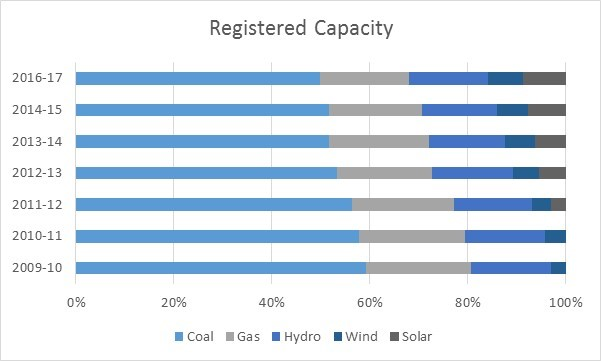
\includegraphics[width=\textwidth]{Registered_capacity.jpg}
    \caption{Registered Capacity}
  \end{minipage}
  \hfill
  \begin{minipage}[b]{0.45\textwidth}
    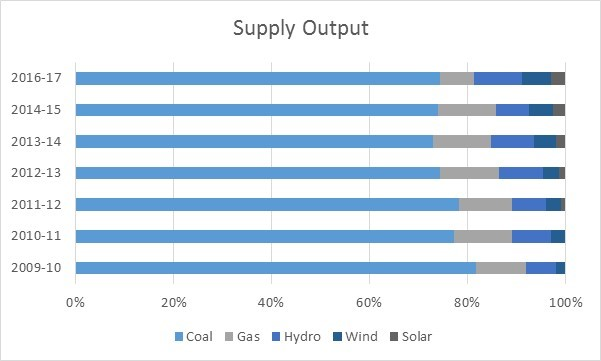
\includegraphics[width=\textwidth]{supply_output.jpg}
    \caption{Supply Output}
  \end{minipage}
\end{figure}
Then the generators make electricity from these sources and flows into the transmission network, which later transports electricity to the distribution network. The distribution network then transports electricity to residential and commercial buildings for end users.\parencite{aemc1}
\begin{figure}[!h]
  \centering
  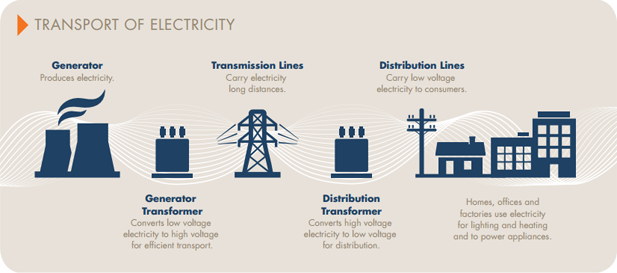
\includegraphics[width=\textwidth]{transport.png}
    \caption{Electricity Transport}
    \parencite{aemo1pic}
\end{figure}
\end{flushleft}
\newpage

\begin{flushleft}
The electricity market in Australia is made up of the following 3 sectors:\par
{\textbf{\large Competitive Wholesale Generation Sector:}}\par
The wholesale national electricity market (NEM) is where generators sell electricity to retailers so they can resell to businesses and households. There are 2 ways in trading electricity in NEM: through spot market or the contract market.\parencite{aemc2} The Australian Energy Market Commission (AEMC) overlooks the states and territories participating in NEM by developing and maintaining the Australian National Electricity Rules (NER). The rules are enforced by the Australian Energy Regulator (AER) and the day-to-day management of NEM is performed by the Australian Energy Market Operator (AEMO).\parencite{aemo1} In Victoria, generators include Loy Yang A and B (supply 30\% electricity needs in Victoria), Yallourn W (supply 22\% needs in Victoria and 8\% needs in NEM), and addition capacity is provided by Pelican Point in South Australia, Tamat Valley in Tasmania and Swanbabnk in Queensland. \par
{\textbf{\large Monopoly Network Business:}}\par
The transmission and distribution networks are poles and wires, transformers, switches, monitoring equipment and everything that make up the electricity grid. Given the intensive investment to construct and manage the network, it is cost effective to have a monopoly network service.\parencite{aemc2} In Victoria, the networks are owned by: Ausnet Service, United Energy Distribution, Powercor Australia, Citipower and Jemena.\par
{\textbf{\large Competitive Retail Sector:}}\par
In the retail sector, customers such as businesses and households buy electricity through retailers (e.g. Origin). Some large consumers such as manufactures may purchase electricity straight from wholesale market, i.e. through a generator rather than through a retailer.\parencite{aemc2} In this sector, electricity consumption by end users is distributed as the following:
\begin{figure}[!h]
  \centering
  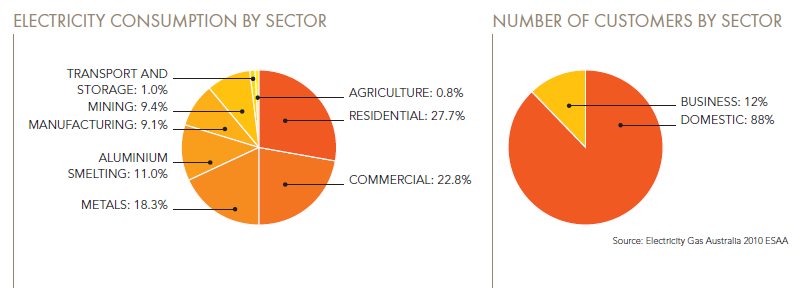
\includegraphics[width=\textwidth]{electricity_consumption.PNG}
    \caption{Electricity Transport}
    \parencite{aemo2}
\end{figure}
\end{flushleft}
\newpage

\subsection{Electricity blackout Compensation}
\begin{flushleft}
Under customers compensation scheme, when end users experience power outages beyond set thresholds, they may be entitled to compensations payments from their electricity distributors in their locations, which are known as "Guaranteed Service Level" payments. However, the amount of payments depends on the nature of events, for example the duration of power interruptions, the number of power interruptions. The payment can go up to \$360 a year.\parencite{cc} \par 
\end{flushleft}

\subsection{Electricity Blackouts in Victoria}
\begin{flushleft}
A power outage, or an electricity blackout is a short-term or a long-term loss of electricity power to a particular area in Wikipedia's definition. As stated in Eaton's Blackout Tracker report, in Victoria about 20 power outages are expected in a year, as taking the average of the number of outages over 2016 to 2018. Also, the average duration of an outage is 199 minutes and 9,923 people are affected per outage in 2018.\parencite{Eaton} Electricity blackouts may be caused by many reasons:
\begin{itemize}
 \item extreme weather (e.g. lighting, floods, heatwaves, bushfires)
 \item falling trees contacting power-lines
 \item animals colliding electricity network equipment
 \item vandalism
 \item underground works, car accident, hot air balloon crash
 \item network overload, equipment failure\parencite{eb2}\parencite{eb1}
\end{itemize}
In Victoria, the leading causes are extreme weather, trees and car accident, with many causes unknown though.\parencite{Eaton} Although it is difficult to put a price on the outages leading to loss of business, one could roughly estimate the cost by valuing what the business would have gained if it were not for the power outage. For example, for a car manufacturer, if it can produce 12,000 cars per day and each car is worth \$50,000, then including the recovery period from the outage, the manufacturer would lose \$600 millions due to one outage. 
\end{flushleft}
\newpage
%%%%%%%%%%%%%%%


%%%%%%%%%%%%%%%
\section{Potential Product Structure}
\begin{flushleft}
This section explain what EBI would seek to achieve for XYZ and its customers, describing a potential structure for the product and explaining the likelihood and severity of electricity blackouts in Victoria.
\end{flushleft}
\fullboxbegin
Note this proposal is a guideline of what should be considered in the product design including definition of an eligible claim and the designated coverage. The actual design is more complex and may involve further investigations. \par
\fullboxend

\subsection{Product Structure}
{\textbf{\large Retail Customers:}}\par
\begin{flushleft}
For retail customers, it might be more attractive to customers to put electricity blackout coverage as an add-on item in their existing household policies. When a retail customers sought electricity blackout insurance, then:
\begin{itemize}
    \item a clear definition of power blackout needs to be established, e.g.:
    \begin{itemize}
        \item unplanned power outages such as outages caused by extreme weather and car accidents, planned outages are not covered
        \item outages caused by vandalism by the insured are not covered
    \end{itemize}
    \item a clear formula for the claim amount needs to be established, e.g.:
    \begin{itemize}
        \item percentage cost of replacing spoiled food over a week for the household;
        \item percentage cost of replacing/repairing damaged electronic devices due to the power surge; 
        \item a formula based entirely on the duration of the power blackout, thereby allowing the insured party to determine the level of cover; or
        \item a formula based on the spike in electricity prices throughout the blackout;
        \item any cost that is not directly related to the outages are not covered, e.g. damage to the fridge caused by spoiled food such as broken seals and stains, or theft and robbery when the alarm system is off during the blackout;
        \item any medical cost and death that are not directly related to the outages are not covered, such as when the life-supporting equipment stop functioning during the blackout which leads to worsen condition or death 
    \end{itemize}
\end{itemize}
\end{flushleft}
{\textbf{\large Commercial Customers:}}\par
\begin{flushleft}
If a commercial enterprise sought power blackout insurance from XYZ, again: 
\begin{itemize}
    \item a clear definition of power blackout needs to be established
    \item a clear formula for the claim amount, e.g.:
\begin{itemize}
    \item percentage of earnings lost and costs of recovering earnings;
    \item a formula based entirely on the duration of the power blackout; or
    \item a formula based on the spike in electricity prices throughout the blackout
period.
\end{itemize}
\end{itemize}

\end{flushleft}
\subsection{Likelihood and Severity}
As mentioned before, the average duration of an outage is 199 minutes 
While the likelihood of an outage could be quite similar although it could be more frequent in area that are more prone to extreme weather such as storms and heatwaves, the severity of damages due to electricity blackout could be quite different depending on the nature of the business. For example, for a supermarket, it could be the spoil frozen food; for a manufacture, it could be the loss of efficiency in production. Hence, the claim amount could be in a wide range and thus the definition of claims needs to be set with intense care.    
Computer systems and other electronic devices containing logic circuitry are susceptible to data loss or hardware damage that can be caused by the sudden loss of power. -> whether they have surge protector
whether they have backup battery 

\newpage
%%%%%%%%%%%%%%%


%%%%%%%%%%%%%%%
\section{Pricing and Risk}
This section describes how the proposed product could be priced and the risks for the insurer XYZ. 

\subsection{Pricing}
\begin{flushleft}
household: rating factors: generator for life-supporting equipment? how many refrigerators? postcode? (area with more cyclones etc.) any medicines stored in refrigerators? does electronic device have surge protector? does the circuit system have surge protector?\par
commercial: depends on the formula chosen for the claim amount; rating factors: size of business, number of employees, profit/production per day, whether backup battery, recovery plan during a outage, how often data are backup\par
On a more granular level, the E Source report found that manufacturers tend to suffer the most from long outages, followed by financial service companies, healthcare, and grocery stores. These industries also face significant losses during short outages and power quality disturbances. Consider a car manufacturer that makes about 1,200 cars a day: The cost for each car is roughly \$50,000. That means just one day offline costs the factory \$60 million.\par
Industries dealing with perishable products, from food to pharmaceuticals, are also vulnerable. In one dramatic example, the loss of power in Puerto Rico in the wake of Hurricane Maria resulted in shortages of medical supplies such as IV bags and some drugs. Puerto Rico pharmaceutical manufacturers produce about 10 percent of all drugs consumed by Americans, according to the U.S. Federal Drug Administration.\par
Food products are perishable at any stage along the supply chain, from manufacture to sale. In Winchester, Virginia, HP Hood installed a 15-MW microgrid at its 150-million gallon milk processing plant as insurance against outages. For Hood, even a brief loss of power could result in the plant shutting down for up to 12 hours to clean and re-sterilize equipment.\par
\end{flushleft}

\subsection{Risk}
\begin{flushleft}
The main risk for the insured is the risk of loss of electricity to the premises being
insured.
The risk for XYZ is the unexpectedly higher payments of claims.
This is caused by higher frequencies of power blackouts and higher inflation on goods
damaged or earnings lost.
\end{flushleft}
%%%%%%%%%%%%%%%


%%%%%%%%%%%%%%%
\section{Relevant Derivatives}
This section outlines the relevant derivative products offered on the Australian Stock Exchange, including how they are quoted and priced, paying particular attention to futures and options in respect of: 
\begin{itemize}
 \item Base - Quarterly
 \item Base - Monthly
 \item Base - Caps
 \item Base - Strip
 \item Peak - Quarterly
\end{itemize}

\begin{flushleft}
https://www.aemc.gov.au/energy-system/electricity/electricity-market/spot-and-contract-markets
https://www.abc.net.au/mediawatch/transcripts/1234_aemo2.pdf
\end{flushleft}

\begin{table}[!h]
\centering
\caption{Sample table.}
\begin{tabular}{cccc}
\toprule
Value 1 & Value 2 & Value 3 & Value 4\\
\midrule
 odd     & odd   & odd & 1.00 \\
 even    & even  & even& 1.00 \\
 odd     & odd   & odd & 1.00 \\
 even    & even  & even& 1.00 \\
\bottomrule
\end{tabular}
\end{table}
%%%%%%%%%%%%%%%

%%%%%%%%%%%%%%%
\section{Liabilities Management}
Indicate how these could be used to manage XYZ’s EBI liabilities, giving a simple numerical example. \par

\frameboxbegin{Example: using derivatives to manage liabilities}
give a numerical example
\frameboxend
%%%%%%%%%%%%%%%

%%%%%%%%%%%%%%%
\section{Residual Risks Management}
Give some residual risks for XYZ and indicate how they could be managed. 
%%%%%%%%%%%%%%%

%%%%%%%%%%%%%%%
\section{Conclusion}
Give a conclusion on whether it is worthwhile XYZ pursuing an EBI offering, in whatever form. 
%%%%%%%%%%%%%%%
\newpage
\printbibliography[heading=bibintoc]
\end{document}          
